\documentclass[10pt, french, a4paper]{report}

\usepackage{babel}
\usepackage{fontspec}
\usepackage{graphicx}
\usepackage{titlesec}
\usepackage{tikz}
\usepackage[hidelinks]{hyperref}
\usepackage{amsmath}
\usepackage{todonotes}
\usepackage{calc}
\usepackage{enumitem}

\newfontfamily{\codefont}{JetBrains Mono}[Scale=0.85]
\setmainfont[Ligatures={TeX, Common, Rare, Historic}]{Linux Libertine}

\newcommand{\class}[1]{{\codefont \NoAutoSpacing \mbox{#1}}}

\titleformat{\chapter}
	{\normalfont\LARGE\bfseries}{\thechapter.}{1em}{}

\tikzset{every picture/.style={execute at begin picture={
   \NoAutoSpacing;}
}}


\title{
	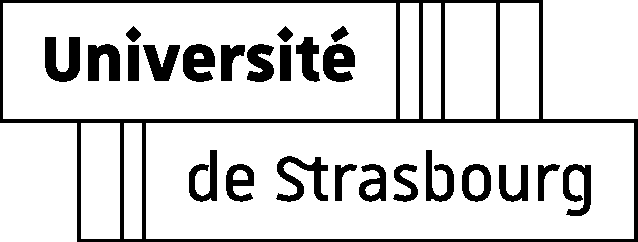
\includegraphics[width=0.5\textwidth]{logo-uds.pdf}\\
	\vspace{2em}
	Master~1 -- Image et 3 Dimensions\\
	Projet de Programmation Avancée\\
	Rapport Final
}
\author{Maxime \textsc{Hohl}}
\date{5 mai 2020}


\begin{document}

\maketitle

\tableofcontents

\chapter{Design}

Le jeu \textit{Asteroids} est découpé en deux grandes parties, le moteur et le jeu lui 
même. Le moteur est lui même découpé en 3 modules~:
\begin{itemize}
	\item Le module de rendu~: qui s'occupe de l'affichage de différents éléments à l'écran.
	\item Le module de physique~: qui s'occupe des calculs physique, c'est à dire des
	      déplacements et des collisions.
	\item Le module de GUI~: qui s'occupe de l'affichage des éléments d'interface utilisateur.
	\item Le module de particules~: Un système de particules qui ne fonctionne pas encore 
	      dans la version rendue, bien qu'il soit assez avancé d'un point de vue du 
	      développement.
\end{itemize}

Tout les éléments du jeu et du moteur interagissent ensemble grâce au \textit{design pattern} Observateur. Voir la Figure~\ref{fig:design-global}.

\begin{figure}[h]
	\center
	\caption{Design global}
	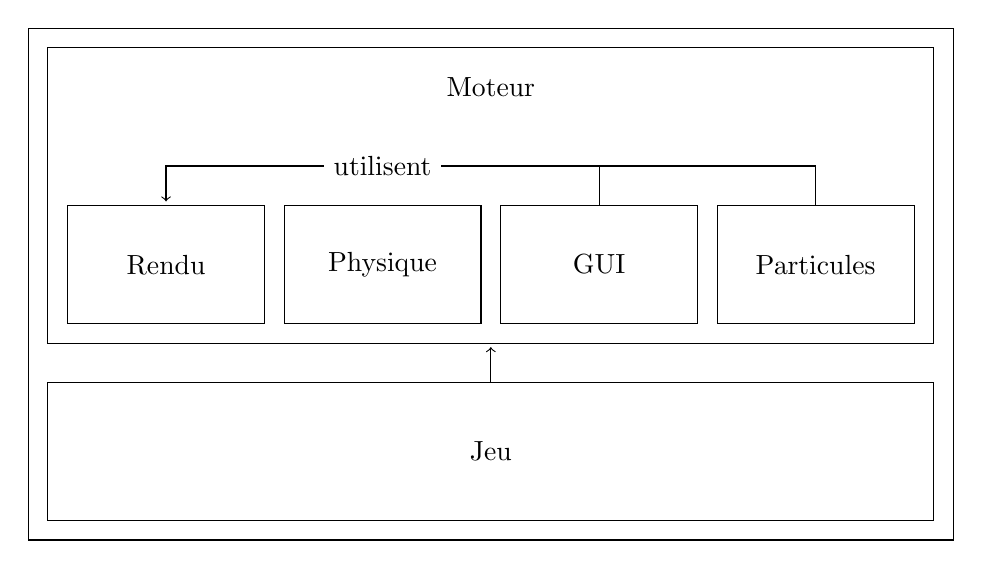
\begin{tikzpicture}	
		\draw (0, 0) rectangle (11.75, 6.5);
	
		
		\draw (0.25, 2.5) rectangle (11.5, 6.25);
		\node at (5.875, 5.75) {Moteur};
		
		\draw (.5, 2.75) rectangle (3, 4.25);
		\node at (1.75, 3.5) {Rendu};
		
		\draw (3.25, 2.75) rectangle (5.75, 4.25);
		\node at (4.5, 3.5) {Physique};
		
		\draw (6, 2.75) rectangle (8.5, 4.25);
		\node at (7.25, 3.5) {GUI};
		
		\draw (8.75, 2.75) rectangle (11.25, 4.25);
		\node at (10, 3.5) {Particules};

		\node (utilise) at (4.5, 4.75) {utilisent};		
		\draw[->] (7.25, 4.25) -- (7.25, 4.75) 
				  -- (utilise) 
				  -- (1.75, 4.75) -- (1.75, 4.30);
		\draw (10, 4.25) -- (10, 4.75) -- (7.25, 4.75);


		\draw (.25, .25) rectangle (11.5, 2);
		\node at (5.875, 1.125) {Jeu};
		
		\draw[->] (5.875, 2) -- (5.875, 2.45);
	\end{tikzpicture}
	\label{fig:design-global}
\end{figure}



\section{Le \textit{design pattern} Observateur}

Ce \textit{design pattern} permet la communication entre les différents éléments du
jeu. Il est composé d'éléments appelés \textit{Observer} qui vont \og recevoir \fg{} 
les messages envoyés par les éléments \textit{Subject} qu'ils observent.

Cf. L'article Wikipedia pour plus d'informations sur le \textit{design pattern}
Observateur~: \url{https://en.wikipedia.org/wiki/Observer_pattern}.

\section{Le module de rendu}

Le module de rendu s'occupe de l'affichage de tout les éléments à l'écran. Il est basé
sur la bibliothèque \textit{SDL2} mais est conçu pour pouvoir la remplacer très 
facilement par un autre système comme \textit{OpenGL} ou \textit{Vulkan}.

Il propose des fonctions de base permettant d'afficher tout les éléments simples 
suivants~:
\begin{itemize}
	\item Des Points
	\item Des Lignes
	\item Des Rectangles vides et pleins
	\item Des polygones quelconques vide
	\item Des Cercle
\end{itemize}

Les modules de GUI et de particules se basent sur lui.

\section{Le module de physique}

Le module de physique s'occupe de tout les calculs physique, c'est à dire, en l'état
actuel des choses, des déplacements en utilisant accélération, vitesse et position 
ainsi que des collisions cercles-cercles, point-cercle et joueur-cercle, le joueur
étant un polygon quelconque bien définis (Voir Figure~\ref{fig:model-joueur}).


\section{Le module de GUI}

Le module de GUI s'occupe de la gestion de tout les éléments d'interface graphique.
En l'état actuel il permet de gérer~:
\begin{itemize}
	\item Des \textit{Panels}~: qui sont de simples rectangles.
	\item Des textes~: qui, aussi surprenant que ça puisse paraitre, sont du texte.
\end{itemize}

Le module à était conçu pour permettre l'ajout de nouveaux éléments d'interface de 
manière assez facile. 

\section{Le module de système de particules}

Ce module ne fonctionne pas encore, mais comme le gros est déjà développé et qu'il 
ressemble à quelque chose, il est présent dans le dossier \textbf{poc/particles} 
mais n'est pas encore utilisé dans le projet.

Il permet de gérer des particules de type point, avec un couleur spécifique.

\section{Le jeu}

Le jeu permet de gérer les astéroïdes au fur et à mesure du temps et en fonction 
du score du joueur. 
Le joueur gagne un point par astéroïde détruit. 

Tout les éléments du jeu reposent sur les différents modules du moteur.


\chapter{Implantation}

L'implantation se s'est faite de manière très directe à partir du design décrit 
précédemment.
Le projet est programmé en \textit{C++17} et repose sur la bibliothèque \textit{SDL2}
qui est en \textit{C} ainsi que sur le système de compilation \textit{CMake}.
Les fichiers sont gérés grâce au système de contrôle de version \textit{git} 
et à \textit{GitLab} (\url{https://git.unistra.fr/m.hohl/projet-progav-maxime-hohl}).

\section{Structure du projet}

Le dossier du projet est découpé en plusieurs sous dossiers~:
\begin{description}[leftmargin=!,labelwidth=\widthof{\bfseries documents}]
	\item [assets] Contient les différents éléments graphiques et audio, c'est à dire 
	               uniquement l'icône du jeu dans le cas présent.
	\item [documents] Contient le présent rapport ainsi que le sujet du projet
	\item [external] Contient les bibliothèques externes essentiels au projet, 
	                 uniquement \textit{SDL2} actuellement.
	\item [include] Contient tout les fichiers \textit{headers} du projet.
	\item [poc] Comme \textit{Proof Of Concept}, contient des modules, morceaux de code 
				ou expérimentations plus ou moins aboutis qui ne sont pas encore intégrés
				le projet.
	\item [src] Contient tout les fichiers \textit{source} du projet.
\end{description}

Les dossiers \textbf{include} et \textbf{src} sont eu-mêmes re-découpés en deux sous dossiers \textbf{Engine} et \textbf{Game} contenant respectivement les fichiers
du moteur et ceux spécifiques au jeu.

\section{Le \textit{design pattern} Observateur}

Toutes les classes qui veulent échanger des donnés doivent hériter de la 
classe \class{Subject} quand elles transmettent des donnés ou de la 
classe \class{Observer} quand elles reçoivent des donnés. Ces deux classes on comme 
paramètre de template le type de donné échangé.

\section{Le module de rendu}

Le module de rendu est constitué d'une classe appelée \class{Renderer} qui 
se base sur \textit{SDL2} mais qui permet de changer aisément pour tout autre 
système en arrière-plan, comme \textit{OpenGL}, \textit{Vulkan}, \textit{Metal}, etc. 


\section{Le module de physique}

Le module de physique est axé sur deux classes principales, 
\class{PhysicEngine} et \\ \class{PhysicEntity}. 
La première effectue tout les calculs liés à la physique et 
tous les objets qui doivent êtres inclus dans les calculs physiques doivent hériter
de la seconde.

Le calcul des mouvements des objets se basent sur les trois formules simples suivantes~:
\begin{align}
	a_t &= a_0\\
	v_t &= v_{t-\Delta t} + a_t * \Delta t\\
	r_t &= r_{t-\Delta t} + v_t * \Delta t
\end{align}
Avec $a$ l'accélération, $v$ la vitesse et $r$ la position, $a_0$, $v_0$ et $r_0$,
respectivement l'accélération initial, la vitesse initial et la position initial 
et $\Delta t$ le temps écoulé depuis le dernier rafraichissement du système 
de physique.

Le système de collision ne permet actuellement que de détecter des collisions du type
cercle-cercle, cercle/point et cercle/joueur.

Les collisions cercles/joueur sont gérés de manière assez particulières. 
Le joueur est un polygone concave quelconque (voir Figure~\ref{fig:model-joueur}), 
il faudrait donc utiliser un algorithme d'intersection entre cercle et polygone concave,
mais ces algorithmes sont assez compliqués et complexes, et en observant bien la 
forme do polygone joueur et la différence de taille entre le joueur et les cercles 
(ici, les astéroïdes), on se rend compte que l'on peut tout simplement effectuer un 
test de collision entre le cercle et les trois points \og extérieurs \fg{} (les points 
cerclés de rouge sur la Figure~\ref{fig:model-joueur}) du polygone et si un point est 
dans un cercle alors il y a collision entre cercle et joueur.

\begin{figure}[h]
	\center
	\caption{Le polygone du joueur}
	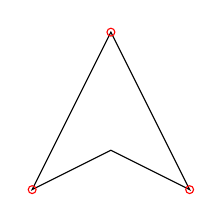
\begin{tikzpicture}[scale=-.5]
		\draw (0, -2) -- (2, 2) -- (0, 1) -- (-2, 2) -- cycle;
		
		\draw[red] (0, -2) circle (0.1cm);
		\draw[red] (2, 2) circle (0.1cm);
		\draw[red] (-2, 2) circle (0.1cm);
	\end{tikzpicture}
	\label{fig:model-joueur}
\end{figure}


\section{Le module de GUI}

Le module de GUI tourne autour des classes~:
\begin{itemize}
	\item \class{gui::Gui} qui est la classe de base de gestion des 
	      éléments d'interface. C'est elle qui gère le rendu et qui doit être
	      utilisée pour créer tout les éléments d'interface.
	\item \class{gui::Entity} qui est la classe virtuelle pure dont tout
		  les éléments d'interface doivent hériter.
\end{itemize}

Chaque entité est positionnée relativement à son parent et à son ancrage. 
Les entités sans parent sont placées par rapport à la fenêtre, toujours en fonction
de l'ancrage (voir Figure~\ref{fig:gui-positionement}).

\begin{figure}[h]
	\center
	\caption{Le positionnement des éléments d'interface. Chaque élément est représenté avec son point d'ancrage. Les éléments vert et rouge ont pour parent l'élément blue, et ce dernier à pour parent la fenêtre (en noir).}
	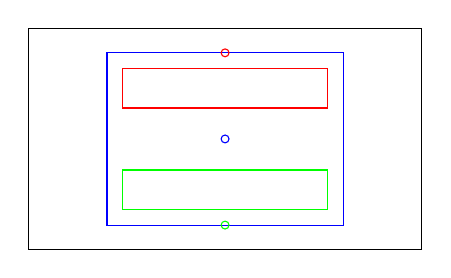
\begin{tikzpicture}		
		\draw (0, 0) rectangle (5, 2.8125);
		
		\draw[blue] (1, .3125) rectangle (4, 2.5);
		\draw[blue] (2.5, 1.40625) circle (0.05cm);
		
		\draw[green] (1.2, .5125) rectangle (3.8, 1.0125);
		\draw[green] (2.5, .3125) circle (0.05cm);
		
		\draw[red] (1.2, 1.8) rectangle (3.8, 2.3);
		\draw[red] (2.5, 2.5) circle (0.05cm);
		
	\end{tikzpicture}
	\label{fig:gui-positionement}
\end{figure}

Chaque entité va se dessiner en appelant des fonctions de la classe
\class{GUIRenderer} puis appeler la fonction de rendu de ses enfants.
Donc si l'on se représente les éléments d'interface via un arbre grâce à leur
lien de parenté, le rendu se fait dans un ordre de parcoure en profondeur, ce
qui permet de garantir que les parents sont toujours rendus avant leur enfants (et sont
donc affichés derrière). Voir Figure~\ref{fig:gui-ordre-rendu}.

\begin{figure}[h]
	\center
	\caption{Ordre de rendu des éléments graphiques
			 (le numéro représentant l'ordre d'affichage)}
	\begin{tikzpicture}[]
		\node{Root}
			child { node {1} 
				child { node {2} }
				child { node {3} }
			}
			child { node {4} }
			child { node {5} 
				child { node {6} 
					child { node {7} }
					child { node {8} }
				}
				child { node {9} }
			};
	\end{tikzpicture}
	\label{fig:gui-ordre-rendu}
\end{figure}

Ce module est le plus aboutit de tous, il ne dispose pas de beaucoup d'éléments
différents, mais il conçu de tel sorte qu'en ajouter un est extrêmement aisé.
Il suffit de créer une classe qui hérite de \class{gui::Entity} 

\section{Le module de système de particules}
 
Pour ce modulen je me suis fortement inspiré de système proposé sur la page suivante~:
\url{http://archive.gamedev.net/archive/reference/articles/article1982.html}.
L'idée est de définir les particules et leur mise à jour grâce à des classes
passées via les templates.

Il y a une classe \class{ParticleEmitter} qui permet d'émettre des particules et qui 
est paramétré avec des classes héritant de \class{InitializationPolicy}, 
\class{UpdatePolicy} et \class{Particle}. 
Les classes \class{BaseXXXXXX} sont des implantations simples de ces classes de base et
sont utilisées comme paramètre par défaut de \class{ParticleEmitter}.

En l'état actuel, le module n'est pas viable, les temps de calculs étant très aléatoires,
allant d'un temps raisonnable à plusieurs secondes. D'autres problèmes semblent
exister, mais faute de temps le module a été délaissé (bien que je compte le reprendre
à titre personnel en me basant peut-être sur les \textit{Compute Shader} 
d'\textit{OpenGL}).

\section{Le jeu}

Le jeu en lui même est axé autour des trois classes suivantes~:
\begin{itemize}
	\item \class{Game}~: qui gère toute la logique du jeu, c'est à dire la boucle
		  principale, les appels de rendu, la gestion des évènements la créations
		  des différents éléments du jeu, etc.
	\item \class{Player}~: qui gère toute la logique derrière le joueur, c'est à dire
		  ses déplacements, et ses tirs.
	\item \class{Asteroids}~: qui gère tout les astéroïdes, de leur création au cours
		  du temps et en fonction du score du joueur à leur destruction si ils sont
		  touchés par des tirs du joueur. 
\end{itemize}

\section{Optimisations}

Toutes les fonctions sont conçues de la manière la plus optimisée possible, mais
aucune passe d'optimisation n'a été effectué. Cela n'était pas nécessaire, étant
donné que le programme tourne à 77 images par secondes constantes sur \textit{Debian~10} 
avec \textit{KDE} et \textit{X11} et à 60 images par secondes constantes sur 
\textit{Windows~10}, les deux avec le système suivant~:
\begin{itemize}
	\item Intel(R) Core(TM) i5-8500 CPU @  3.00GHz, 6 coeurs
	\item 32Go de RAM DDR4
	\item NVIDIA GeForce GTX 1060 6GB
\end{itemize}
On remarquera cependant que les valeurs d'images par secondes ne sont sans doutes pas représentatives car étant donné les valeurs, elles doivent êtres limités par une 
synchronisation vertical. Mais elles permettent quand même de se rendre compte qu'il
n'y a pas de ralentissement dans les temps de rafraichissements et donc pas de forte
nécessite d'optimisation.

\chapter{Problèmes rencontrés et voies d'amélioration}

\section{Problèmes rencontrés}

Au cour du développement du projet, ne nombreux problèmes ont fait surfaces. 
Par exemple, le développement à commencé en considérant des astéroïdes de 
formes quelconques, mais après avoir eu beaucoup de difficultés (et pas assez de 
temps pour les surmonter) pour gérer les collions entre eux, ils sont devenus de 
simples cercles.
Le module de particules m'a aussi donné pas mal de fil à retordre.

\section{Bogues connus}

En l'état actuel, le projet présente trois bogues connues~:
\begin{itemize}
	\item Le jeu \og crash \fg{} quand un astéroïde avec un vitesse de $[0, 0]$ entre en 
	      collision avec le tir d'un joueur. Ce bogue n'est pas urgent à corriger
	      étant donné que les astéroïdes ont une vitesse minimal supérieur à $0$.
	\item Le jeu \og crash \fg{} lors de la collision entre un astéroïde et un tir de
	      joueur quand le projet est compilé avec \textit{MSVC}.
	\item Il arrive que des astéroïdes acquièrent une vitesse beaucoup trop élevée, ce
	      qui les rends quasiment impossibles à éviter.
\end{itemize}

\section{Voies d'amélioration}
\label{sec:voies-amelioration}

J'ai de très nombreuses idées de  voies d'amélioration pour le projet, donc je ne détaillerai que les quartes plus importantes.

La  première concernant le module de physique. Il devrait gérer de manière générique
toutes les entités et non pas spécifiquement les astéroïdes, tirs et joueurs et devrait 
permettre de gérer les collisions entre polygones convexes, ce qui permettrait des 
astéroïdes avec des formes plus folkloriques.

La seconde concerne le visuel. Un module de particules fonctionnel devrait permettre 
d'ajouter du dynamisme au jeu, par exemple en ajoutant des particules à la sortie du 
moteur du vaisseau du joueur ou lors de l'explosion d'un astéroïde. On peut aussi 
envisager de passer sur du rendu purement \textit{OpenGL} pour permettre plus de 
flexibilité sur les effets visuels, comme des distorsions ou des tremblements de 
l'écran lors d'une explosion.

La troisième voie d'amélioration que j'ai envisagée est l'audio. 
L'ajout de musiques et d'effets sonores devrait ajouter un peut de vie dans le jeu.

Enfin, un vrai module de gestion des évènements permettrait de rentre le moteur 
réutilisable.



\chapter*{Conclusion}
\addcontentsline{toc}{chapter}{Conclusion}

Le projet était très intéressant, développer un jeu de zéro (en dehors de \textit{SDL2})
a été très instructif pour moi. J'ai axé le développement du projet plus sur le 
moteur que ce soit en utilisant la puissance du \textit{C++17} ou en essayant
de bien le concevoir que sur le jeu en lui même. C'est pourquoi je me retrouve
avec un des modules que je trouve très aboutis, comme le module de GUI et d'autres 
bien pensés comme le module de Particules ou le \textit{design pattern} Observateur 
(bien que les idées de bases ne soit pas de moi).

Si je devait exprimer une seul frustration ce serait de ne pas avoir put passer plus
de temps sur ce projet. Mais je ne me priverait pas d'améliorer le moteur de jeu
en suivant les quelques idées que j'ai cités à la section~\ref{sec:voies-amelioration}.

\end{document}
